\begin{figure}
    \begin{center}
        % 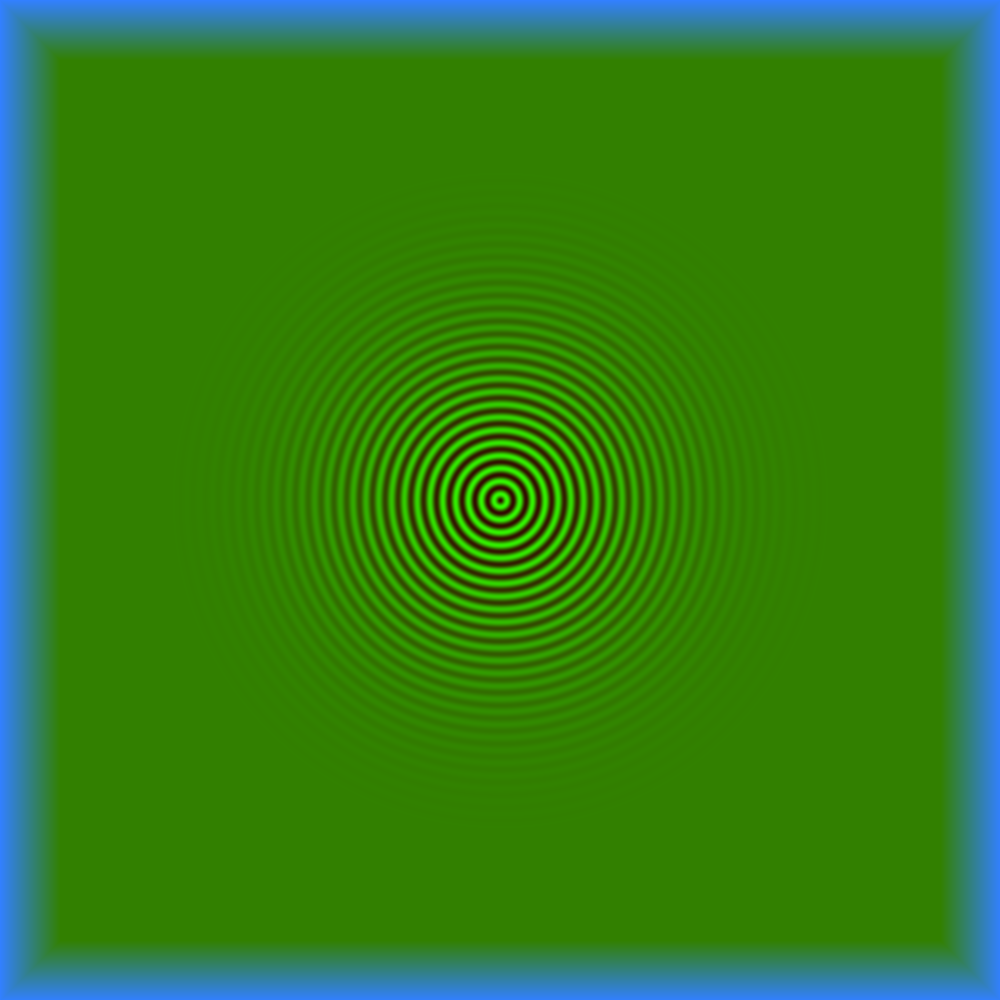
\includegraphics[width=0.5\textwidth]{papers/particles/figures/wavesim/particle_initial_state.png}
        \subfigure[]{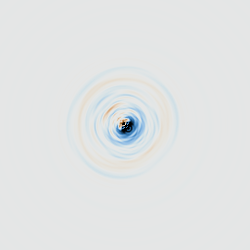
\includegraphics[width=0.45\textwidth]{papers/particles/figures/simulations/particle_frames/frame_12.png}}\hfill
        \subfigure[]{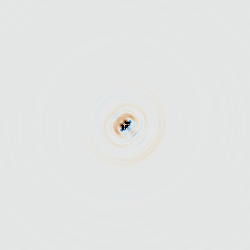
\includegraphics[width=0.45\textwidth]{papers/particles/figures/simulations/particle_frames/frame_13.png}}
        \caption{Asymmetrischer Feldkonfiguration, die entsteht, wenn die gefangenen Energiemenge ausreichend abgenommen hat.}\label{particles:fig:partikel:abnehmen:asymmetrisch}
    \end{center}
\end{figure}